\section{REQUIREMENTS}
\subsection{Functional requirements}
Assuming that the domain assumptions listed in paragraph [\ref{Domain_properties}] hold, and in order to fulfill the goals listed in paragraph [\ref{Goals}], the following requirements can be derived.

Requirements are grouped under each goal from which they are derived. 
\begin{itemize}
	\item {[G1]} Allow users to register to the system by filling out a form. 
	\begin{itemize}
		\item {[R1]} The system will provide a registration form.
		\item {[R2]} The system will allow not registered users to access only the homepage and the registration page.
		\item {[R3]} Upon registration, the system will check the uniqueness of the chosen username. 
	\end{itemize}
	\item {[G2]} Allow registered users to access the system by entering their username and password.
	\begin{itemize}
		\item {[R1]} Registered users must have previously filled out the registration form.
		\item {[R2]} Registered users must have previously received a password via email from the system.
		\item {[R3]} The system will provide a login functionality.
		\item {[R4]} The system will verify the existence of the username-password combination in the database. 
	\end{itemize}
	\item {[G3]} Allow registered users to manage their personal information.
	\begin{itemize}
		\item {[R1]} Registered users must be logged into the system.
		\item {[R2]} The system will provide a personal page for each registered user to manage.
		\item {[R3]} The system will allow registered users to save the personal information they update.
	\end{itemize}
	\item {[G4]} Allow registered users to find the locations of all available cars within a certain distance from their current location or from a specified address.
	\begin{itemize}
		\item {[R1]} Registered users must be logged into the system.
		\item {[R2]} Registered user must have chosen the functionality "make a reservation".
		\item {[R3]} Registered user must have provided a valid address (within the city of Milan), corresponding either to their current location or to a specified address of their choice. 
		\item {[R4]} The system will provide a map showing the location of all the available cars.
	\end{itemize}
	\item {[G5]} Allow registered users to reserve a single car among the available ones in a certain geographical region for up to one hour before they pick it up.
	\begin{itemize}
		\item {[R1]} Registered users must be logged into the system.
		\item {[R2]} Registered users must have chosen the functionality "Make a reservation".
		\item {[R3]} Registered users must have selected a single car among the available ones showed on the map. 
		\item {[R4]} The system must provide a timer that will be activated at the moment of the reservation.
	\end{itemize}
	\item {[G6]} Allow registered users to tell the system they are nearby when they reach a car they previously reserved.
	\begin{itemize}
		\item {[R1]} Registered users must be logged into the system.
		\item {[R2]} Registered users must have selected a single car among the available ones showed on the map. 
		\item {[R3]} The system will provide a mobile functionality that allows the users to unlock the reserved car once they are nearby.
		\item {[R4]} The system will unlock the car once the user is nearby.
	\end{itemize}
	\item {[G7]} Allow registered users to see on a screen the amount of money they are being charged for while they are driving. 
	\begin{itemize}
		\item {[R1]} Each car must have a screen. 
		\item {[R2]} The system will provide a functionality that updates the amount of money the user will be charged of every minute that passes. 
	\end{itemize}
	\item {[G8]} Allow registered users to see on a screen a map showing all the safe areas they can park in. 
	\begin{itemize}
		\item {[R1]} Each car must have a screen.
		\item {[R2]} The car screen will provide an interactive and updated map showing all the safe areas.
		\item {[R3]} The system will provide a functionality that detects the safe areas.
	\end{itemize}
	\item {[G9]} Allow registered users to see on a screen the discount/overcharge percentage (if any) applied on their bill once the ride has ended.
	\begin{itemize}
		\item {[R1]} Each car must have a screen.
		\item {[R2]} The system will be able to realize when a user parks into a safe area.
		\item {[R3]} The system will provide a functionality that calculates the ride price after applying the discount percentage/overcharge.
	\end{itemize}
	\item {[G10]} Allow registered users to cancel a reservation paying a 1EUR fee.
	\begin{itemize}
		\item {[R1]} Registered users must be logged into the system.
		\item {[R2]} Registered users must have previously reserved a car and not yet unlocked it.
		\item {[R3]} The system will provide a functionality that allows registered users to cancel their current reservation.
	\end{itemize}
	\item {[G11]} Allow registered users to benefit from a discount/pay an overcharge percentage in certain cases.
	\begin{itemize}
		\item {[R1]} The system will provide a functionality that calculates the ride price after applying the discount/overcharge percentage.
		\item {[R2]} The system will recognize the cases in which the user is supposed to benefit from a discount/pay an overcharge percentage.
		\item {[R3]} Registered user must have parked in a safe area and turned off the car ignition.
	\end{itemize}
	\item {[G12]} Allow registered users to report an issue when they realize a car they reserved is somehow broken.
	\begin{itemize}
		\item {[R1]} Registered users must be logged into the system.
		\item {[R2]} Registered users must have previously reserved a car.
		\item {[R3]} Registered users must have unlocked the car.
		\item {[R4]} The system will provide a mobile functionality (not web) that allows registered users to report an issue.
	\end{itemize}
	\item {[G13]} Allow employees to interact with the system and manage cars information.
	\begin{itemize}
		\item {[R1]} Employees must be logged into the system.
		\item {[R2]} The system will provide a web functionality (not mobile) that allows employees to manage cars information.
	\end{itemize}
\end{itemize}
\newpage
\subsection{Nonfunctional requirements}
\subsubsection{Mobile interface} 
\begin{itemize}
	\item Homepage:
	\begin{figure}[H]
		\centering
		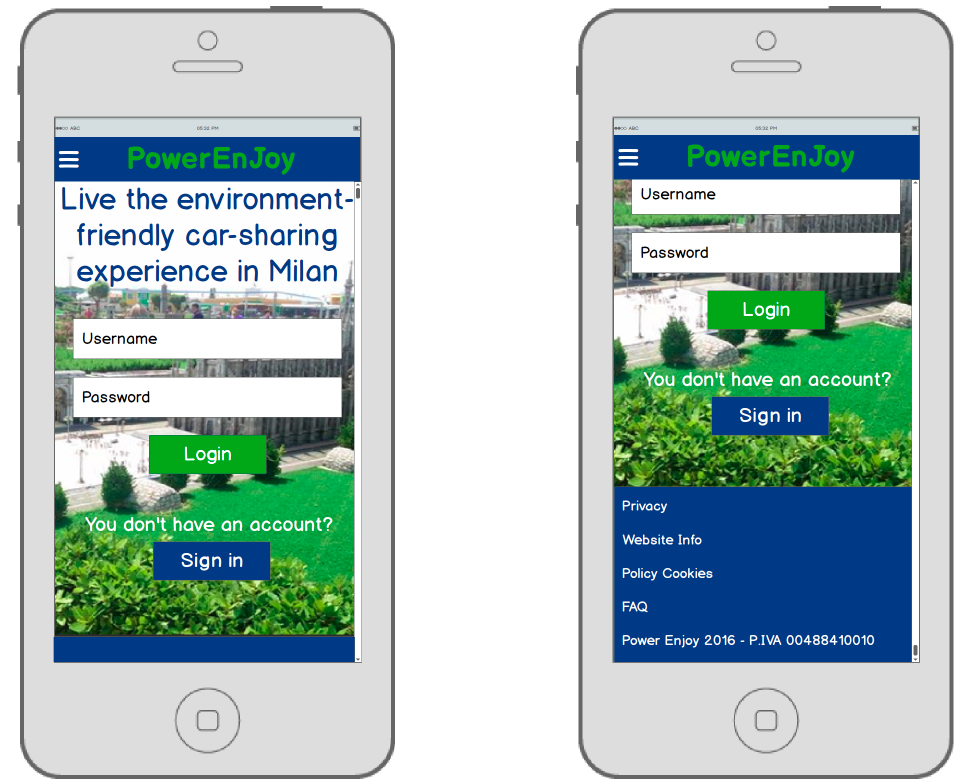
\includegraphics[width=1\textwidth]{Mobile_homepage}
	\end{figure}
\newpage
\item Registration:
\begin{figure}[H]
	\centering
	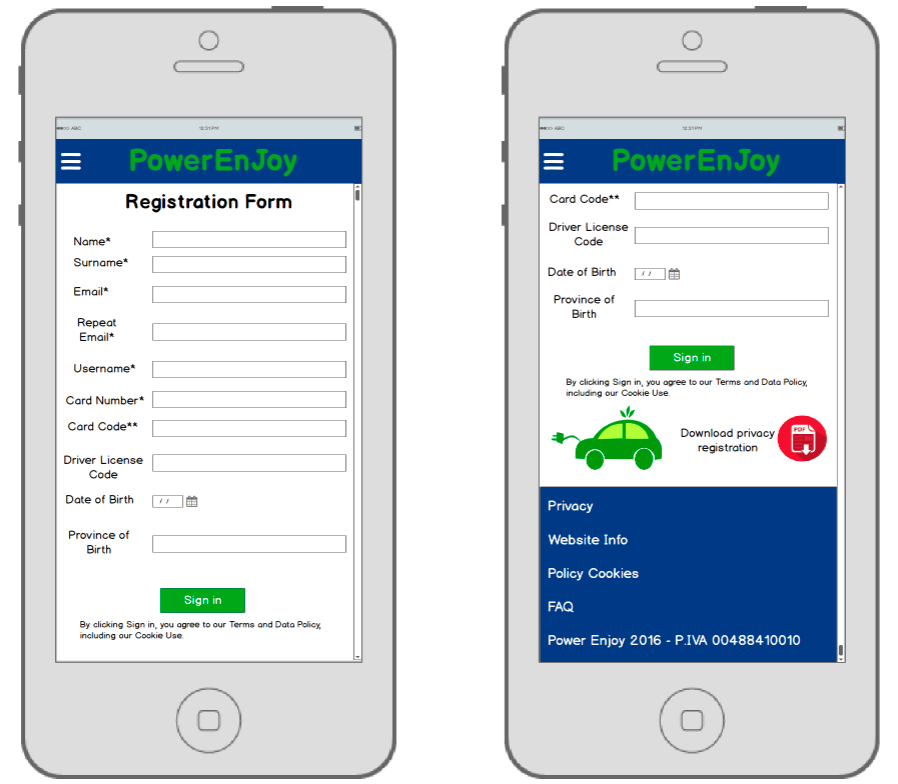
\includegraphics[width=1\textwidth]{Mobile_registration}
\end{figure}
\newpage
\item Receiving the password:
\begin{figure}[H]
	\centering
	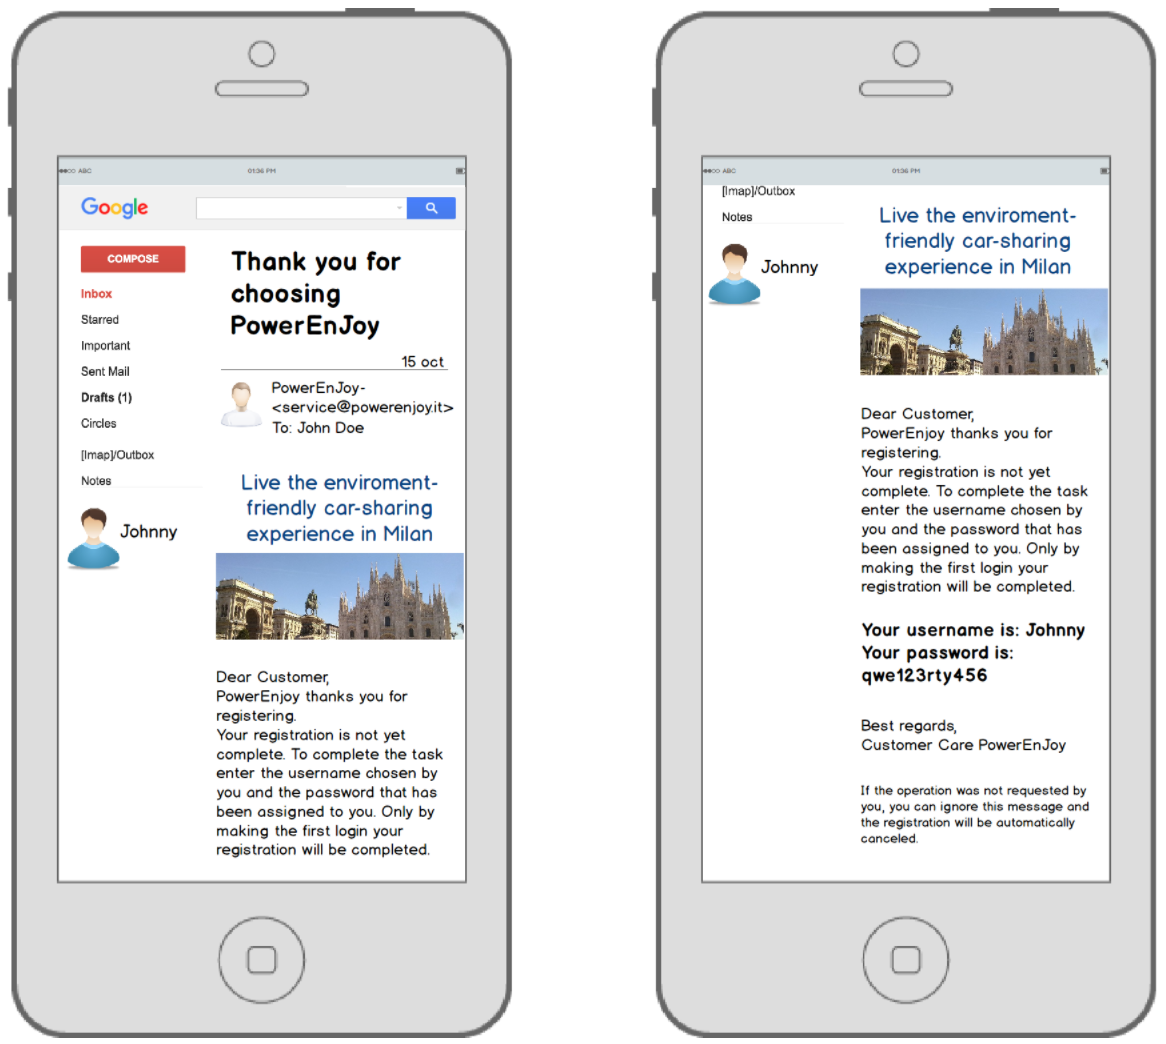
\includegraphics[width=1\textwidth]{Mobile_password}
\end{figure}
\newpage
\item Personal page:
\begin{figure}[H]
	\centering
	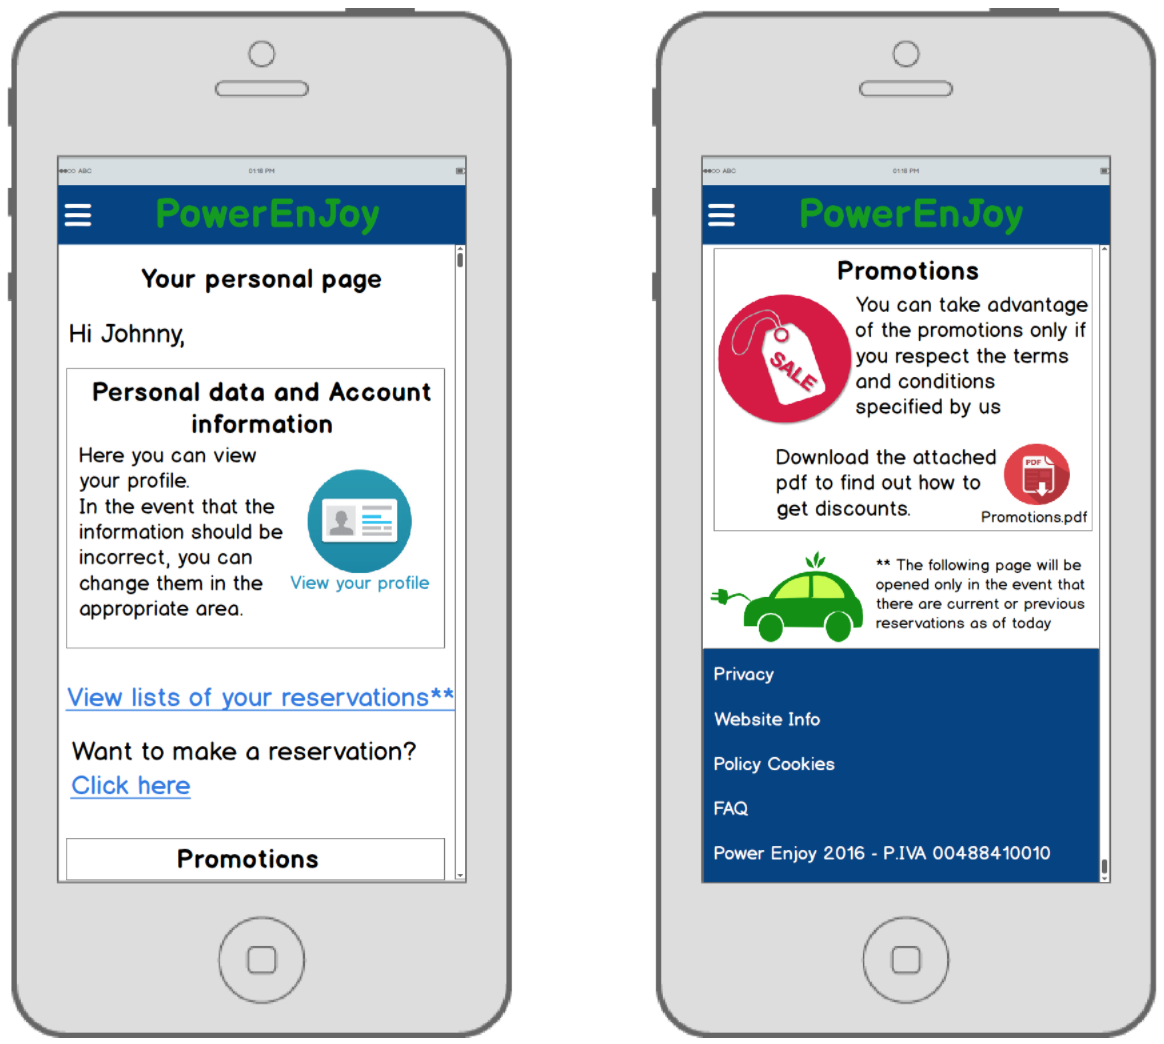
\includegraphics[width=1\textwidth]{Mobile_personal_page}
\end{figure}
\newpage
\item View profile:
\begin{figure}[H]
	\centering
	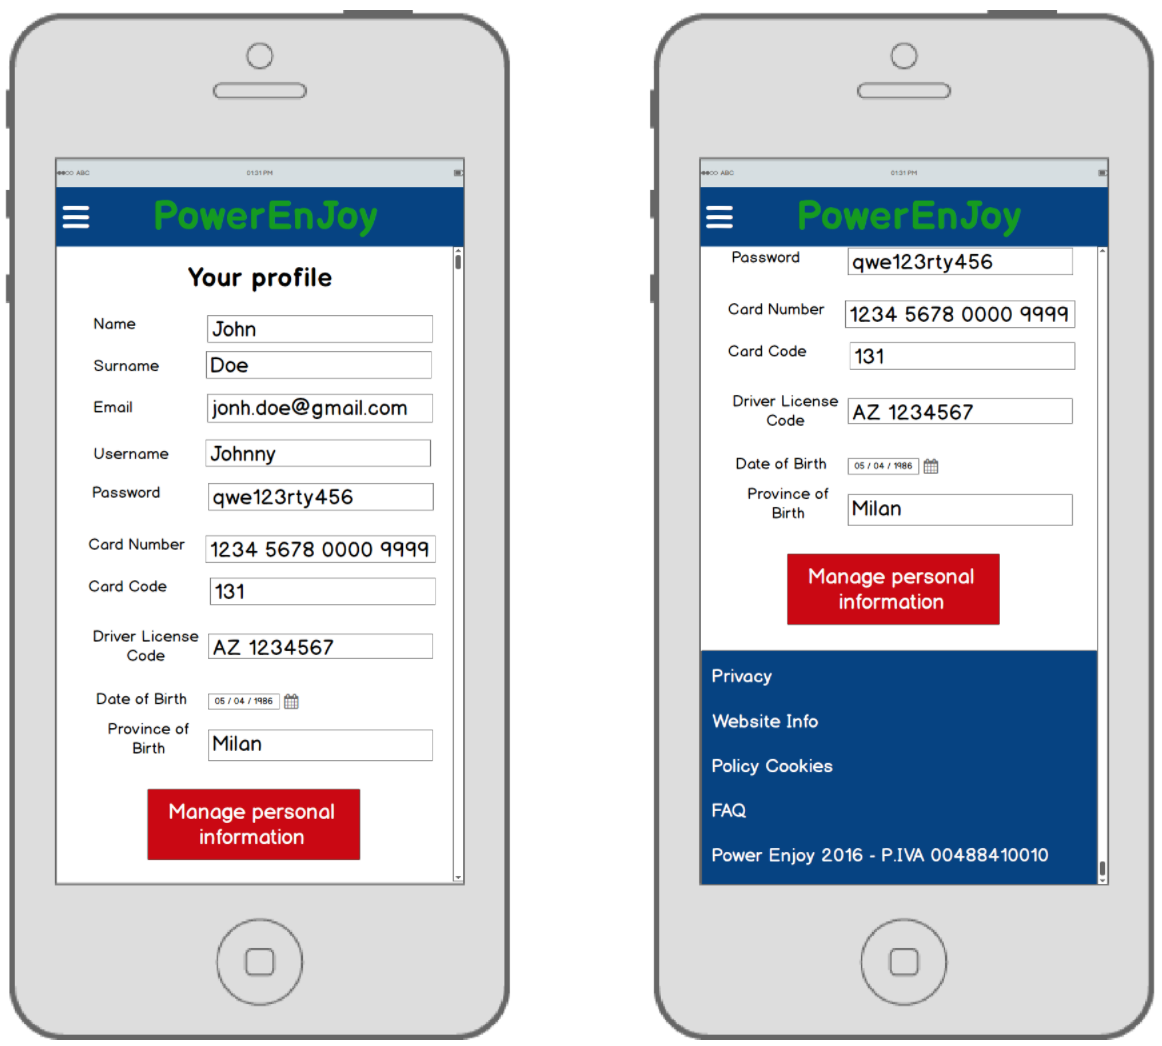
\includegraphics[width=1\textwidth]{Mobile_view_profile}
\end{figure}
\newpage
\item Managing personal information:
\begin{figure}[H]
	\centering
	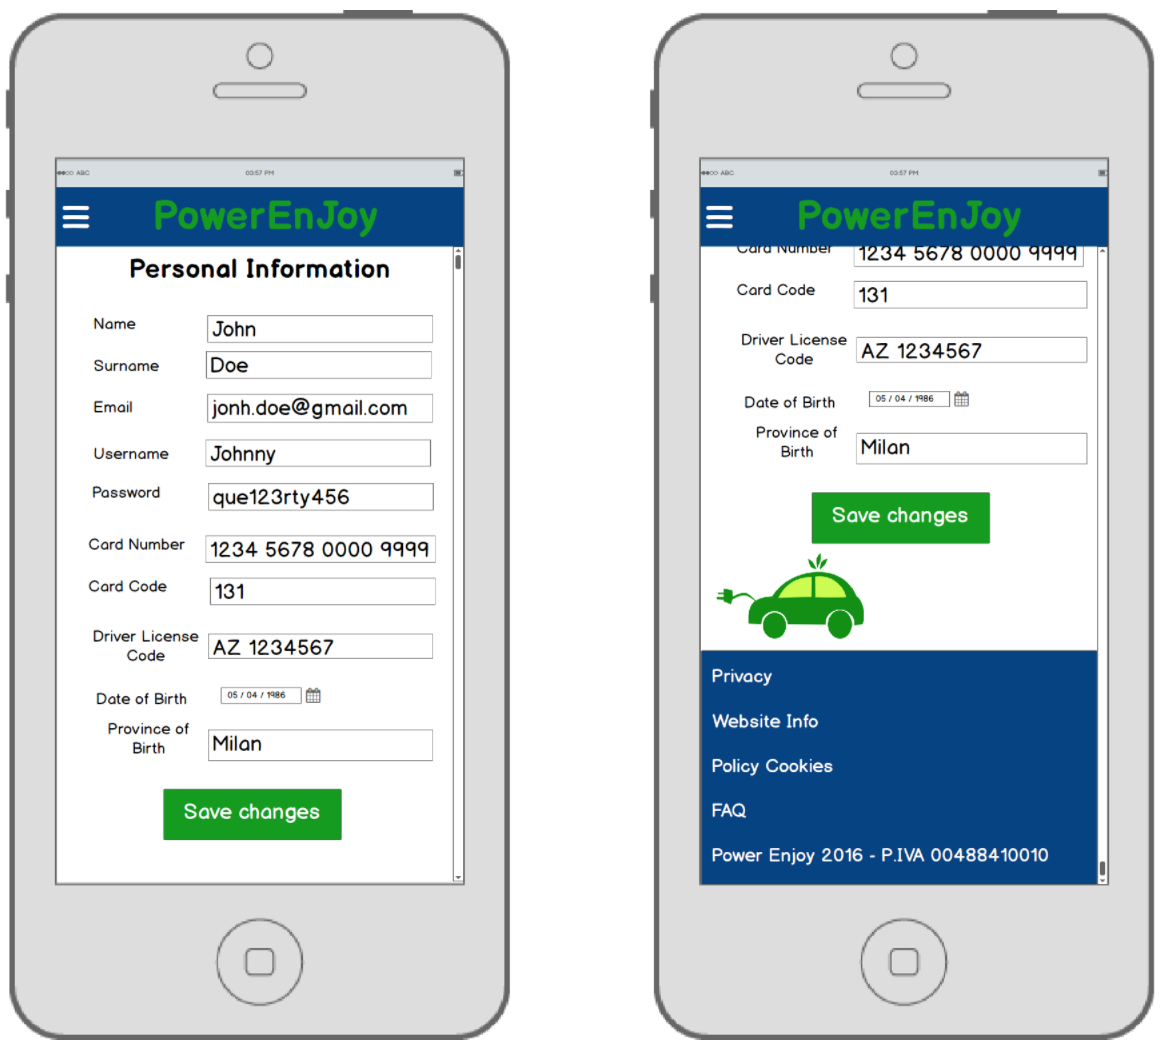
\includegraphics[width=1\textwidth]{Mobile_change_info}
\end{figure}
\newpage
\item Making a reservation:
\begin{figure}[H]
	\centering
	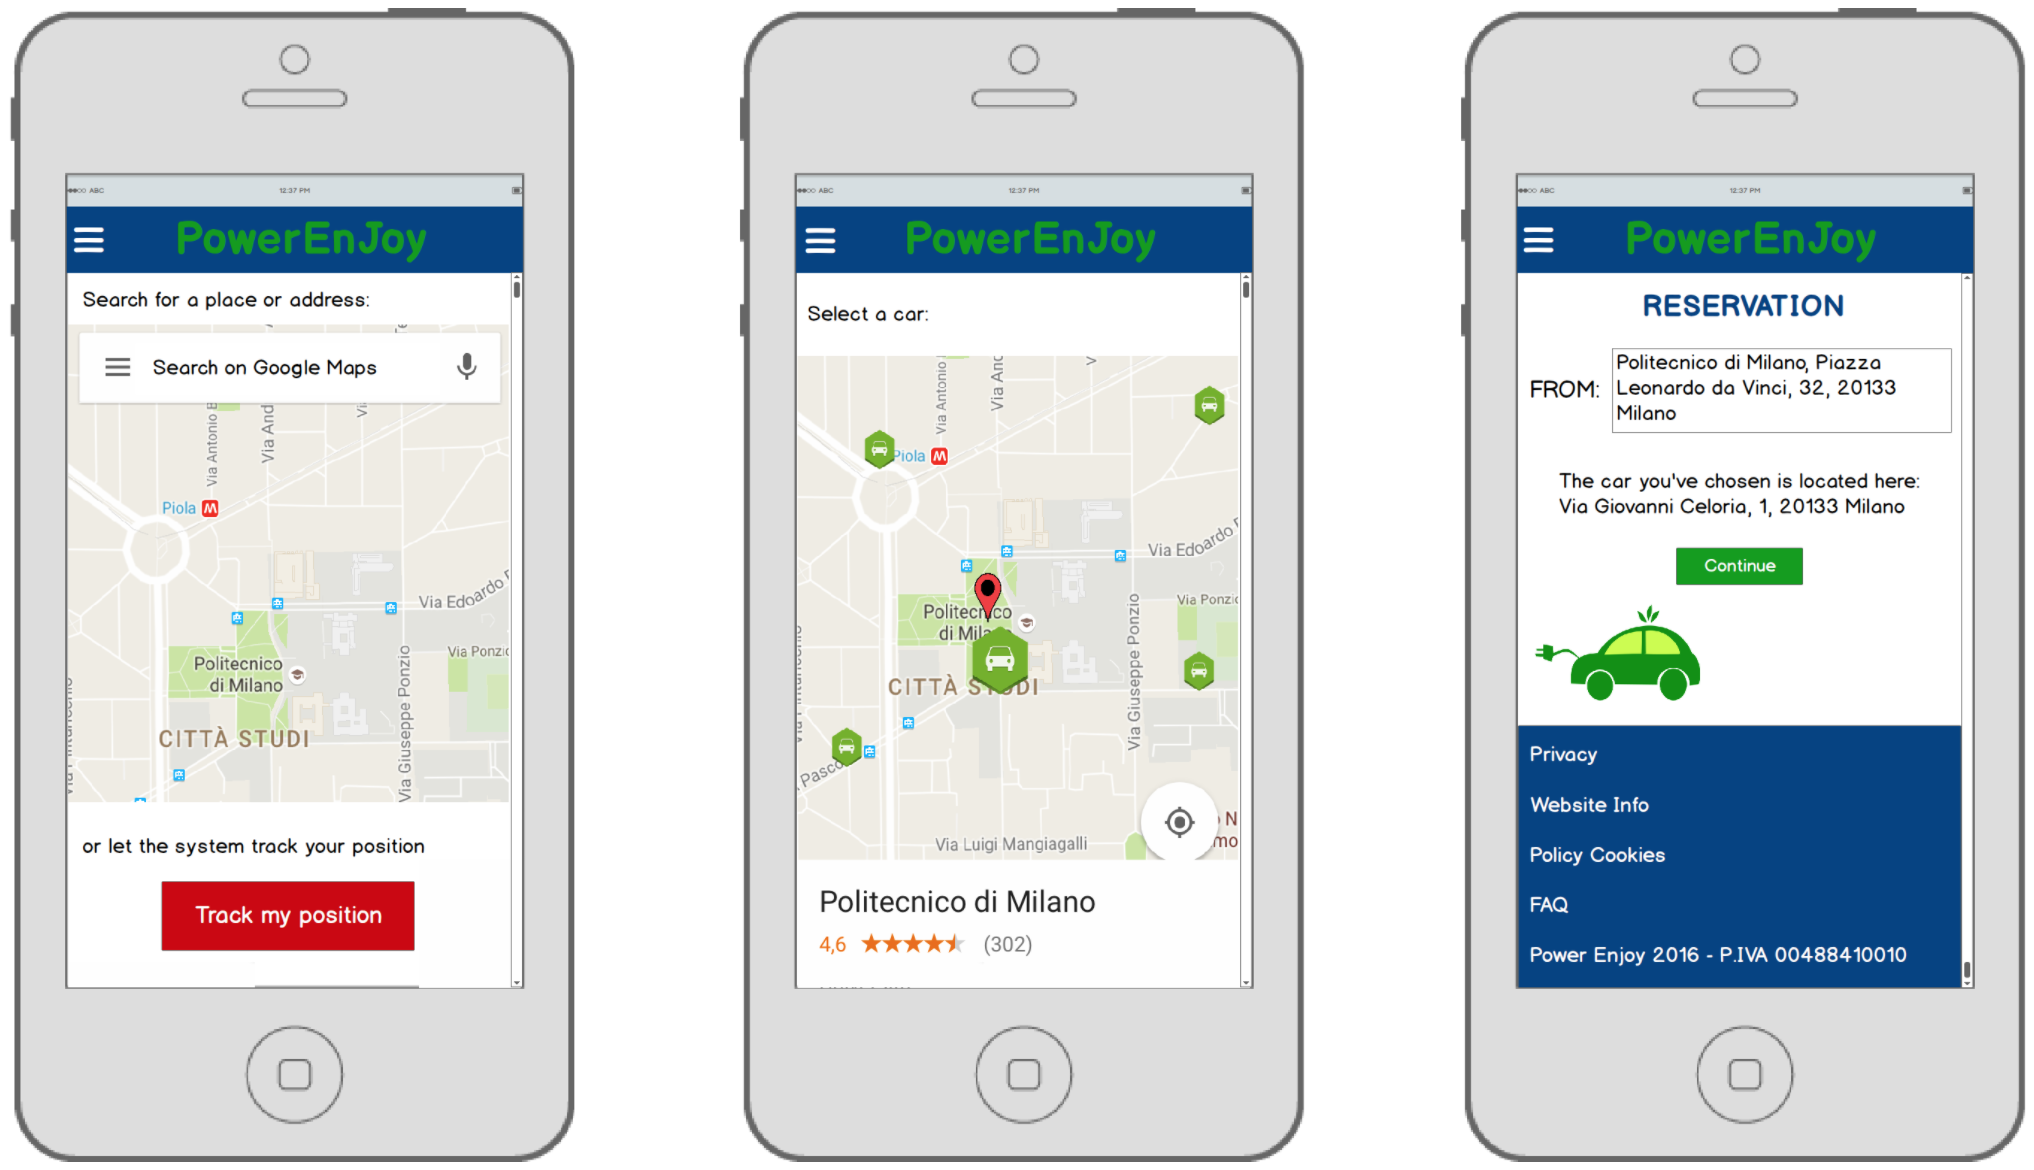
\includegraphics[width=1\textwidth]{Mobile_reservation}
\end{figure}
\newpage
\item Deleting a reservation:
\begin{figure}[H]
	\centering
	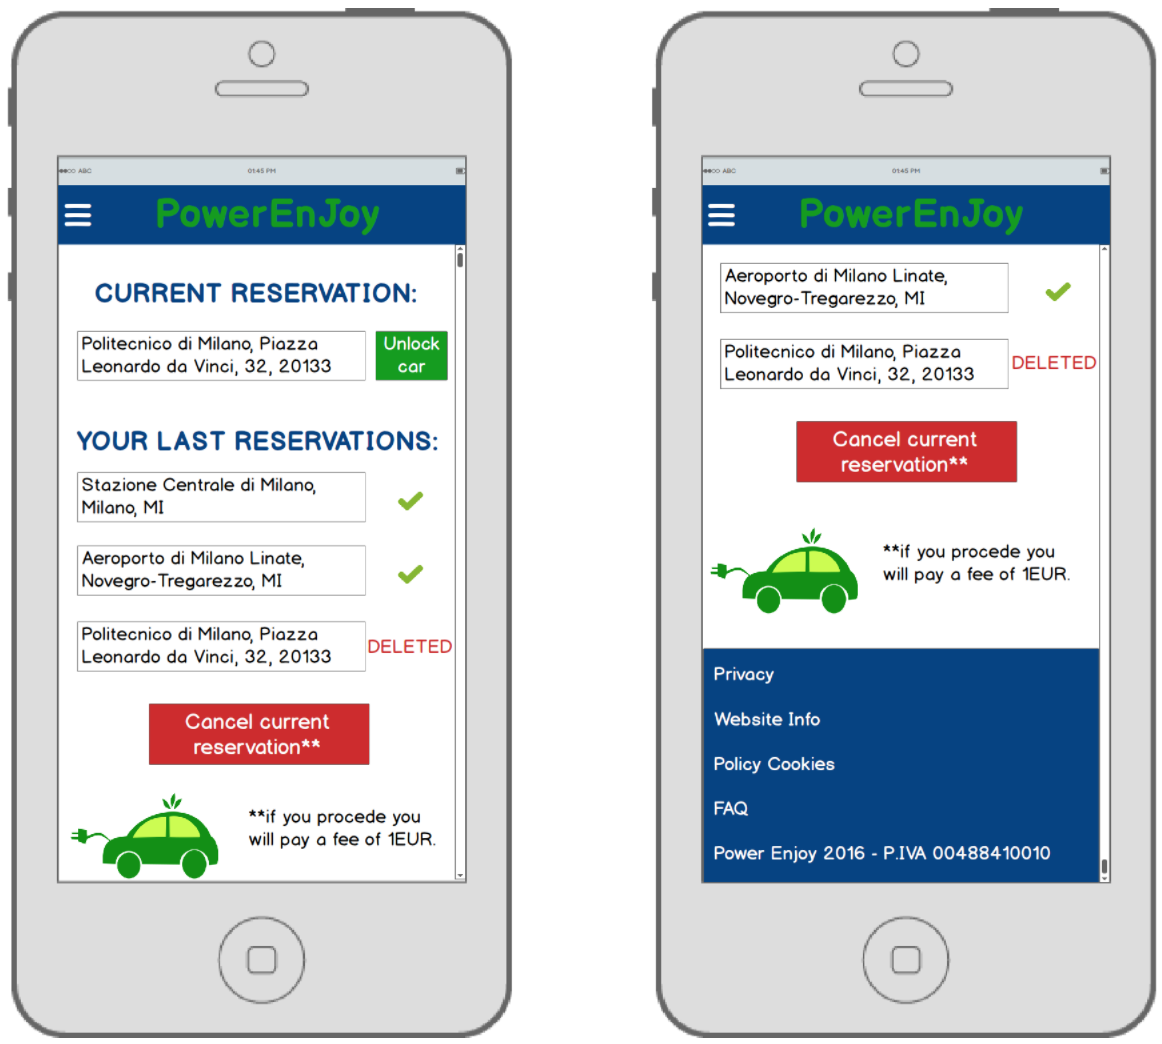
\includegraphics[width=1\textwidth]{Mobile_cancel_reservation}
\end{figure}
\newpage
\item Reporting an issue:
\begin{figure}[H]
	\centering
	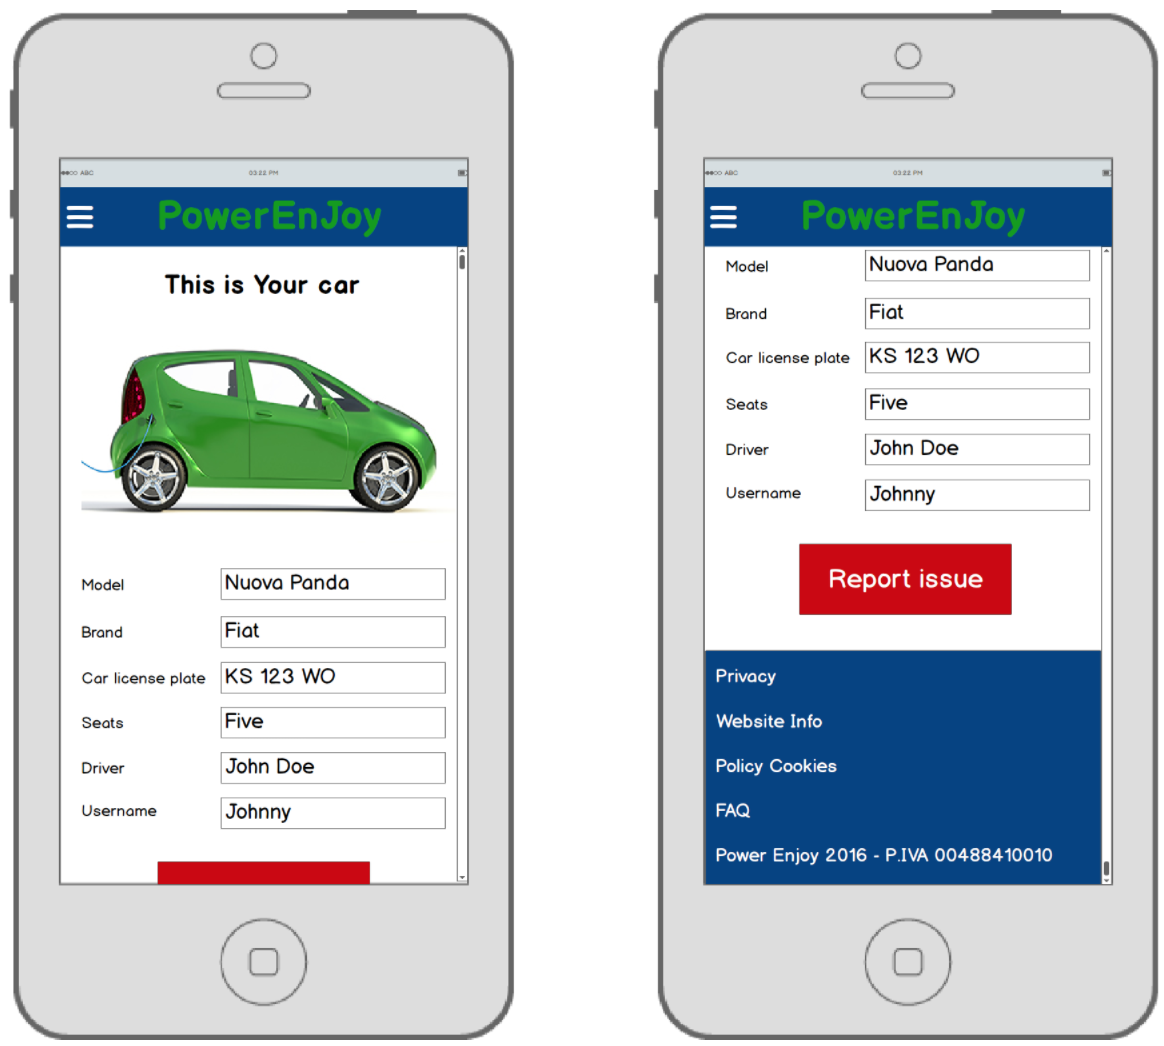
\includegraphics[width=1\textwidth]{Mobile_report_issue}
\end{figure}
\end{itemize}
\newpage
\subsubsection{Web interface}
\begin{itemize}
	\item Homepage: 
	\begin{figure}[H]
		\centering
		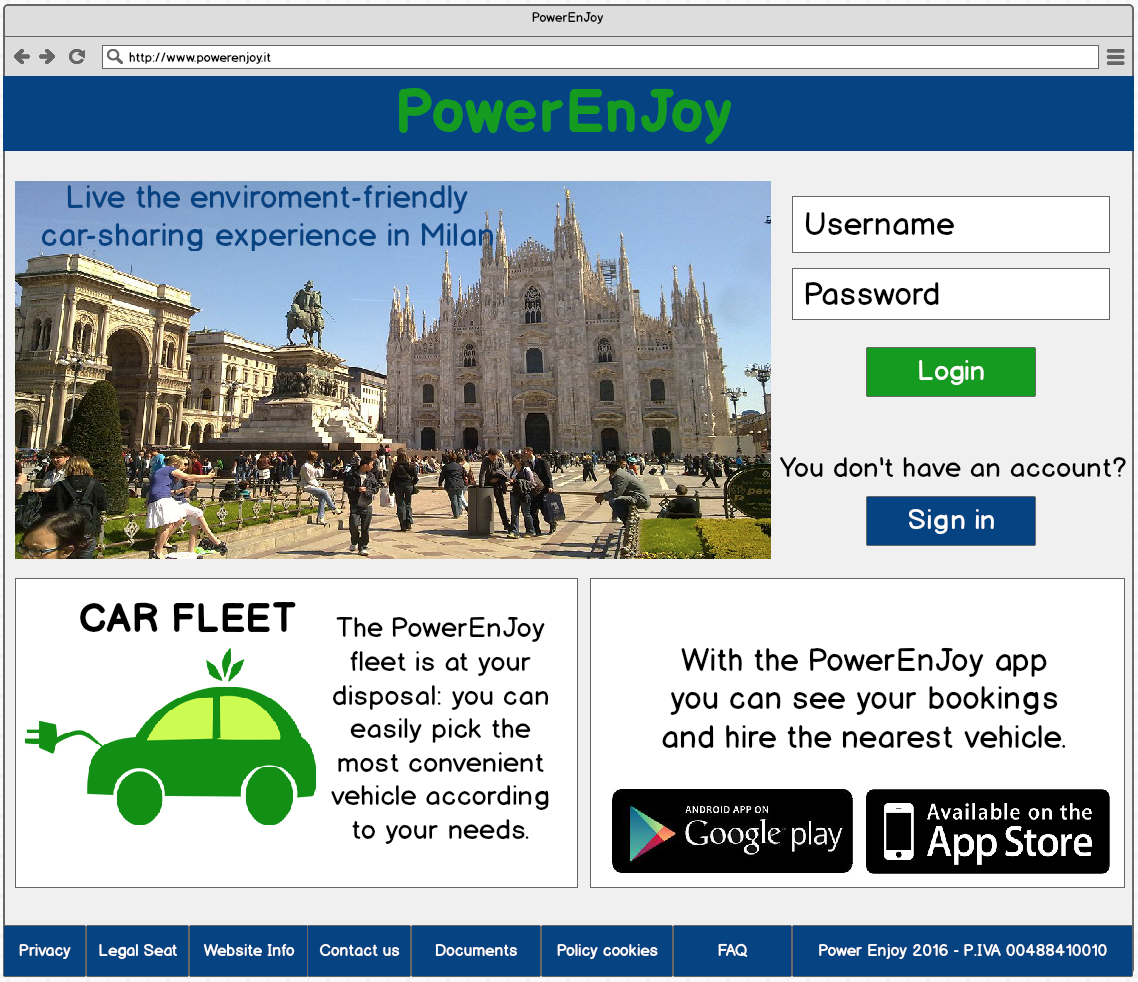
\includegraphics[width=1\textwidth]{Web_homepage}
	\end{figure}
\newpage
\item User registration:
\begin{figure}[H]
	\centering
	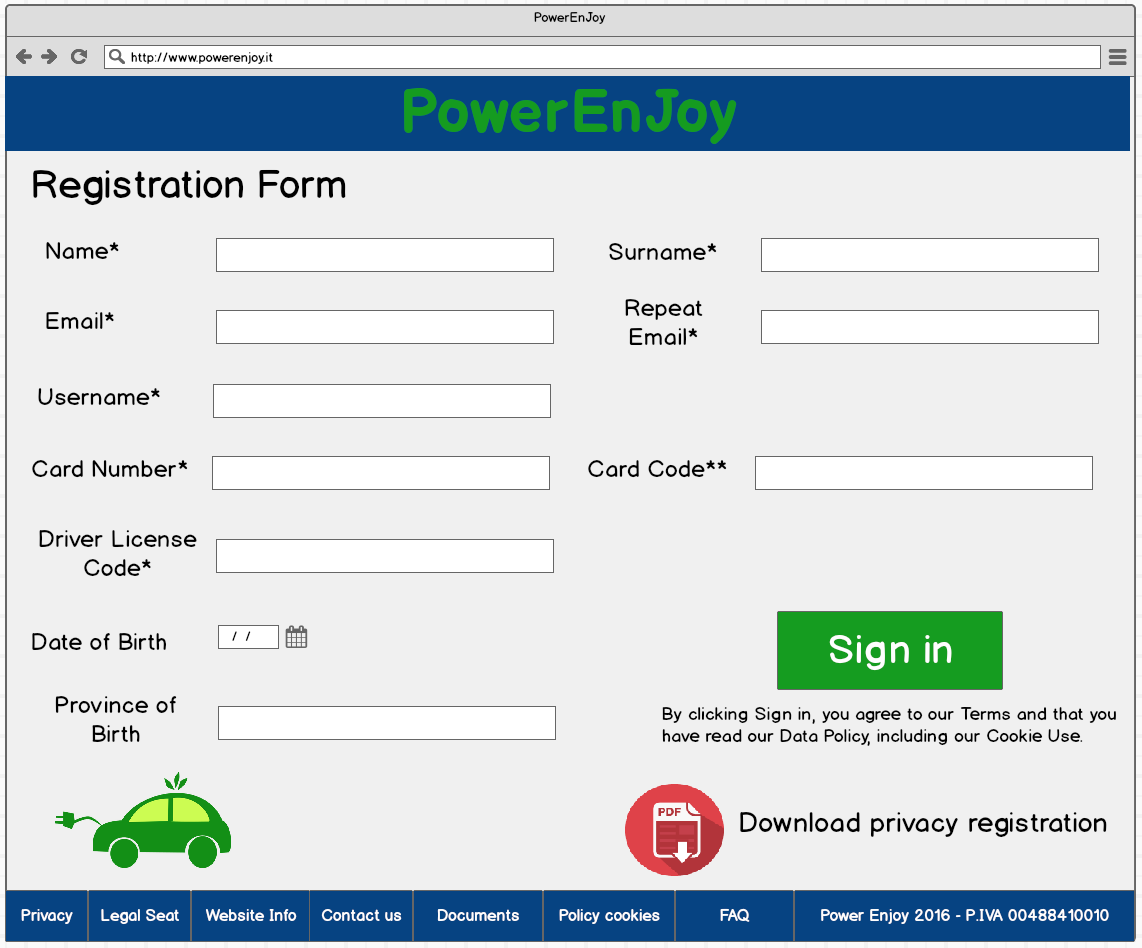
\includegraphics[width=1\textwidth]{Web_registration}
\end{figure}
\newpage
\item User receives the password:
\begin{figure}[H]
	\centering
	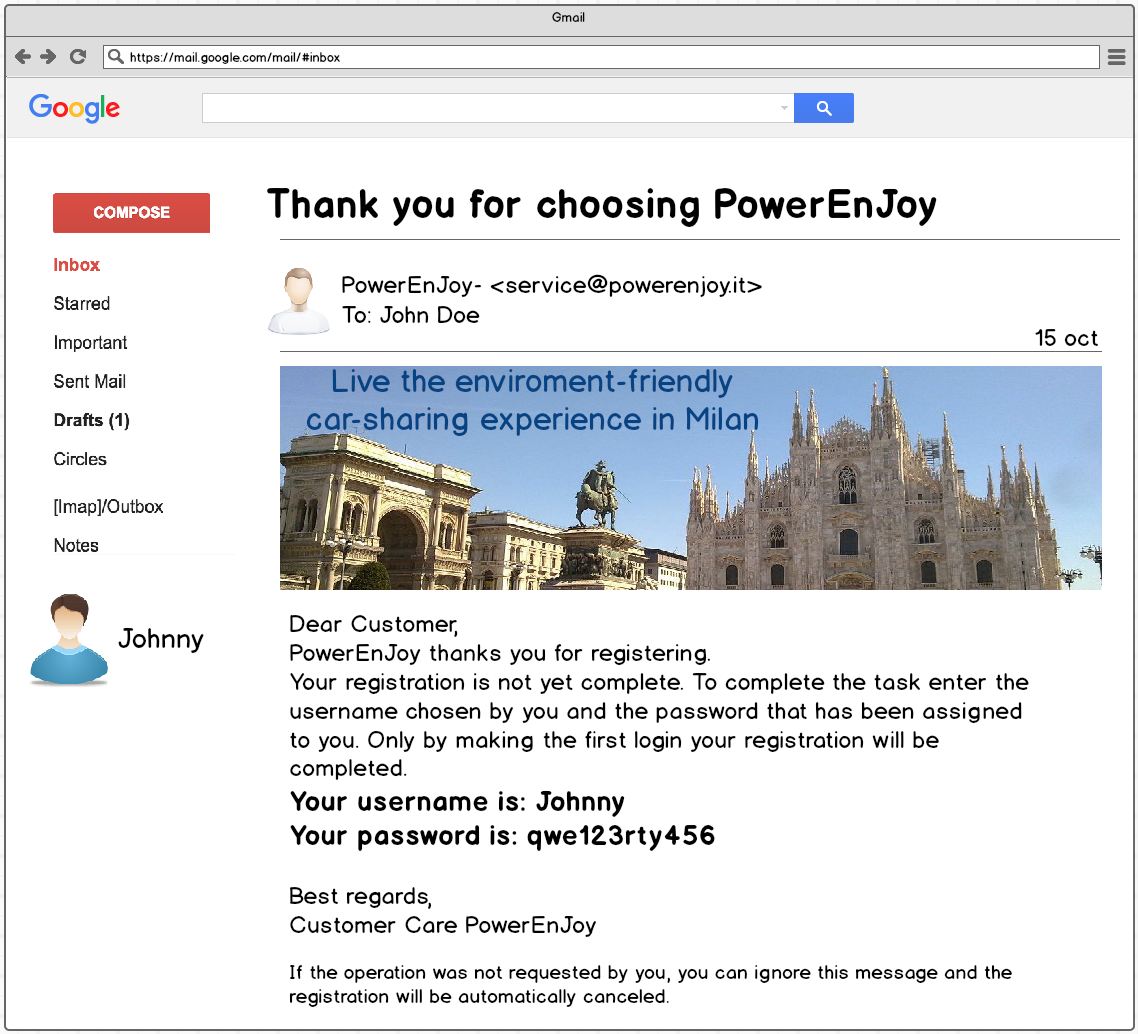
\includegraphics[width=1\textwidth]{Web_password}
\end{figure}
\newpage
\item Registered user's personal page:
\begin{figure}[H]
	\centering
	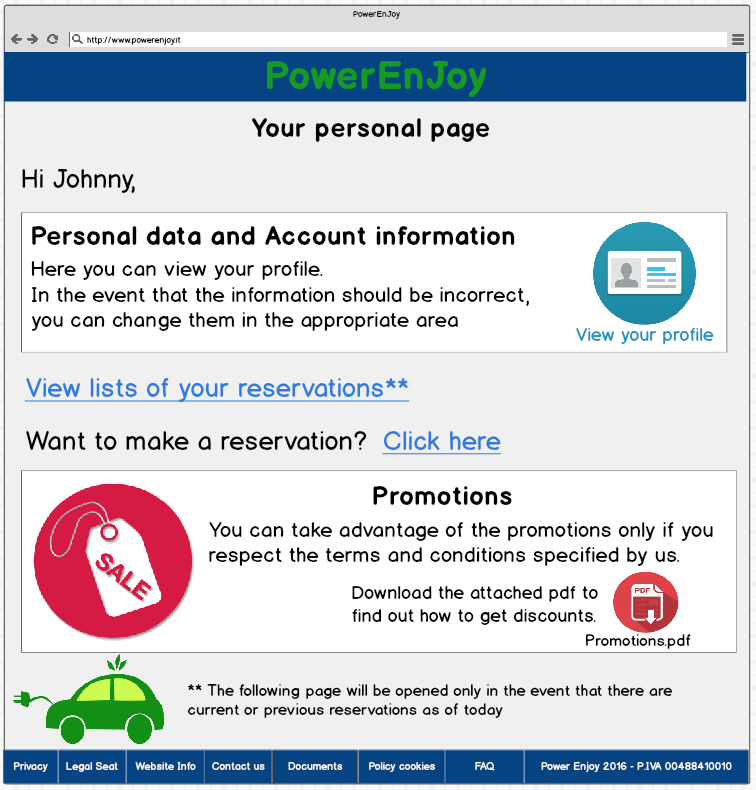
\includegraphics[width=1\textwidth]{Web_personal_page}
\end{figure}
\newpage
\item Registered user's profile:
\begin{figure}[H]
	\centering
	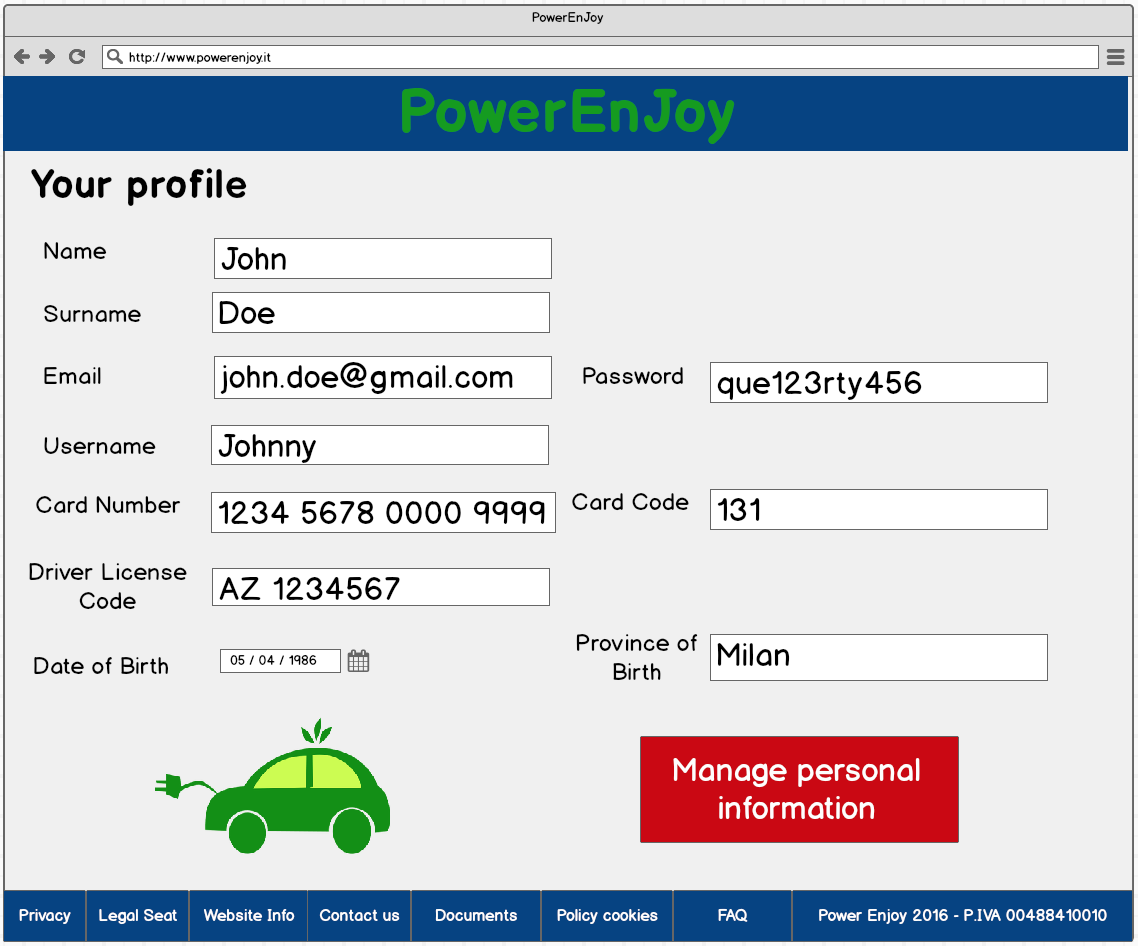
\includegraphics[width=1\textwidth]{Web_view_profile}
\end{figure}
\newpage
\item Registered user manages his/her personal information:
\begin{figure}[H]
	\centering
	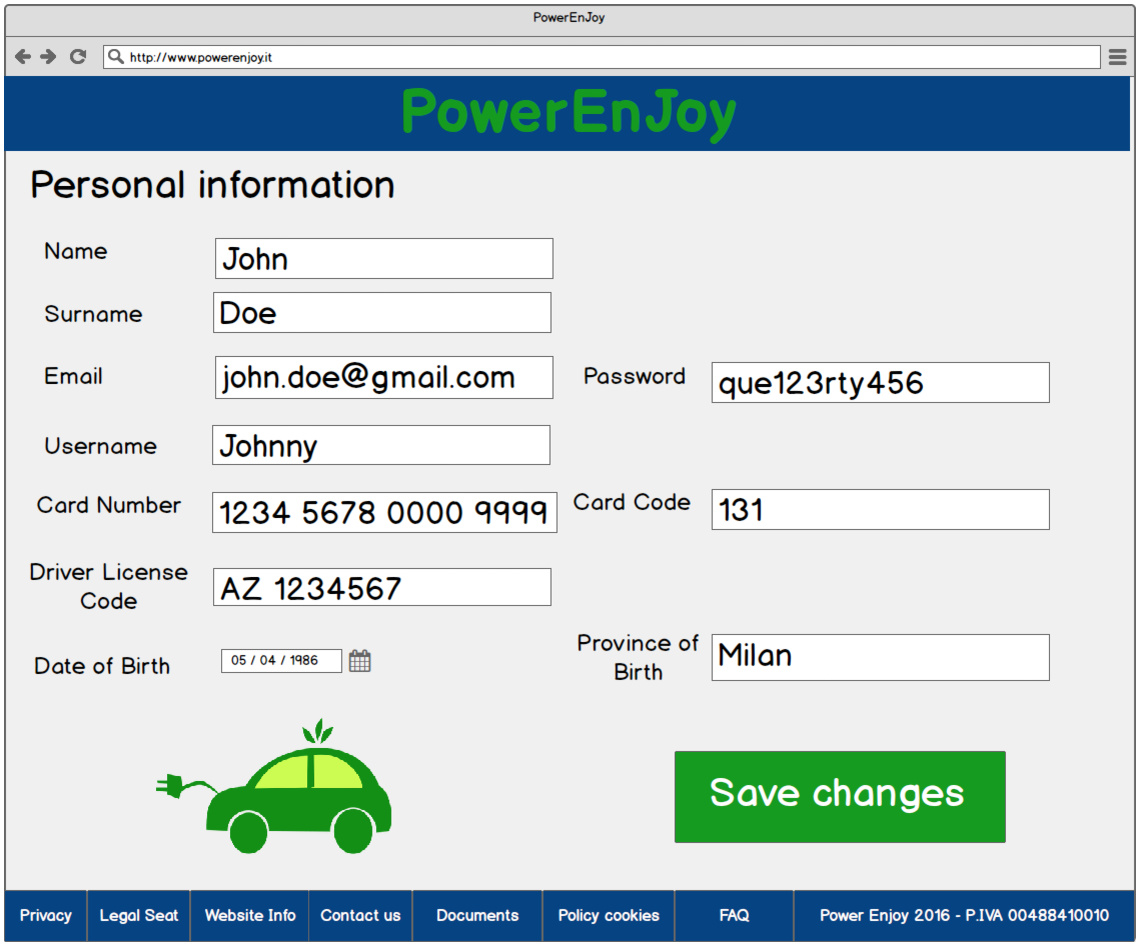
\includegraphics[width=1\textwidth]{Web_change_info}
\end{figure}
\newpage
\item Registered user makes a reservation:
\begin{figure}[H]
	\centering
	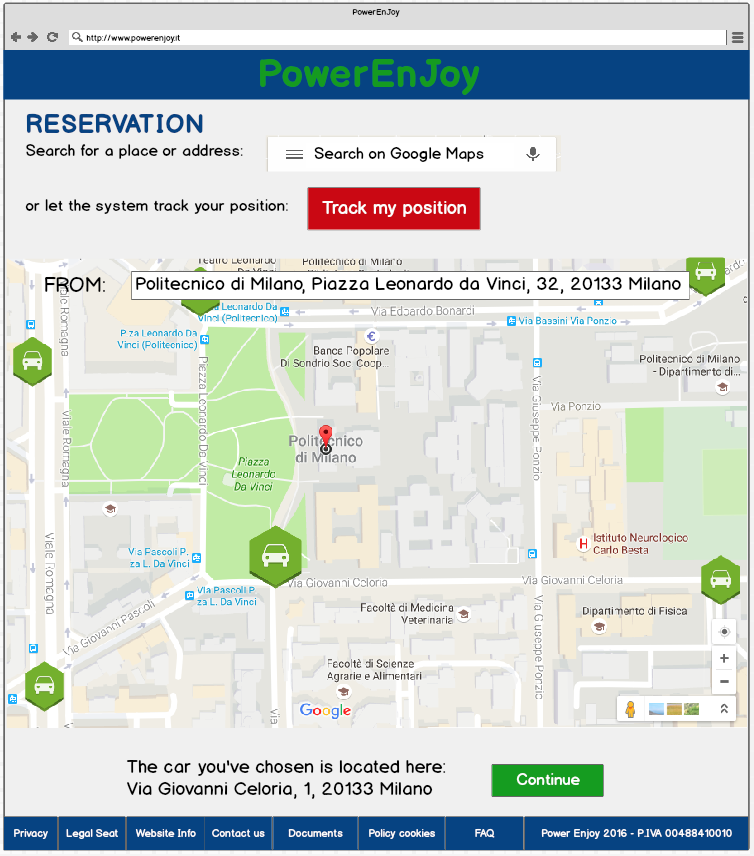
\includegraphics[width=1\textwidth]{Web_reservation}
\end{figure}
\newpage
\item Registered user deletes a reservation:
\begin{figure}[H]
	\centering
	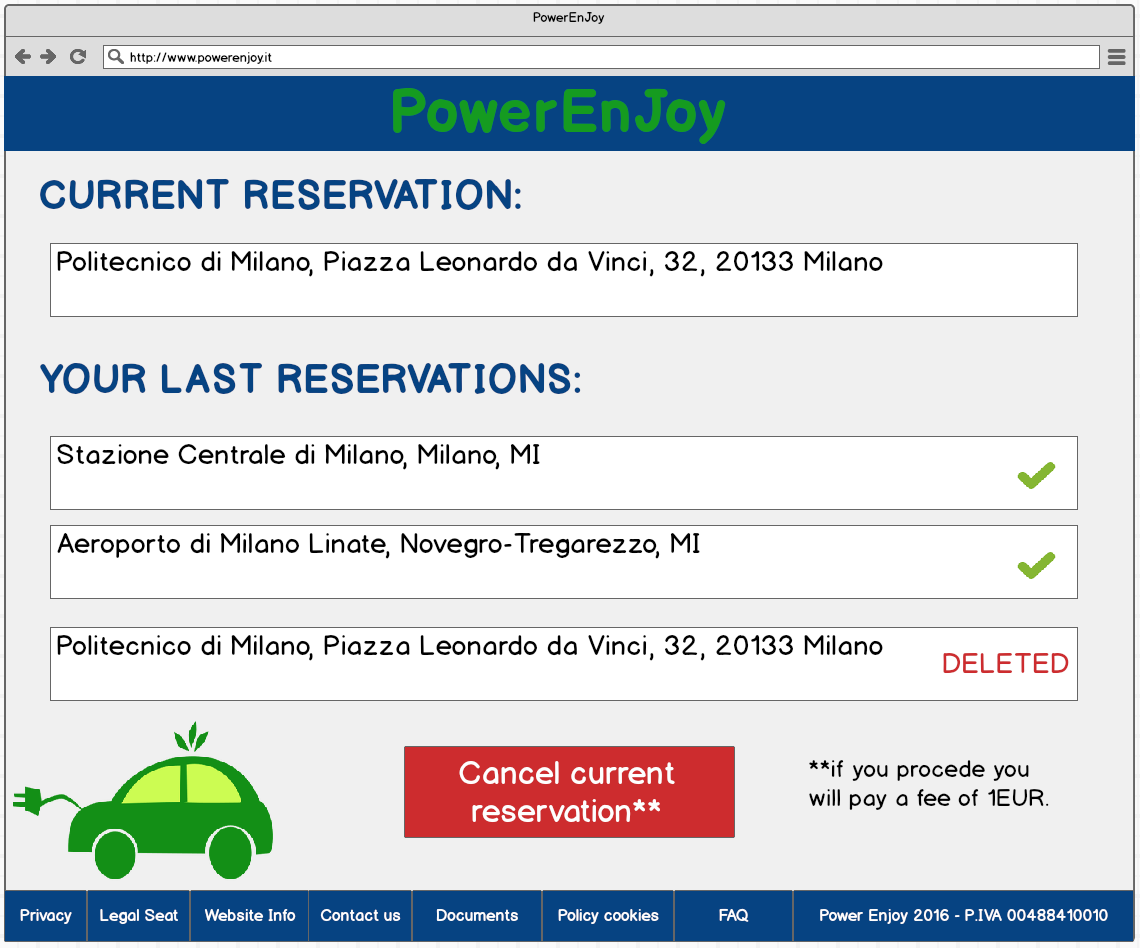
\includegraphics[width=1\textwidth]{Web_cancel_reservation}
\end{figure}
\end{itemize}
\newpage
\subsubsection{Employee}
\begin{itemize}
	\item Employee's personal page:
	\begin{figure}[H]
		\centering
		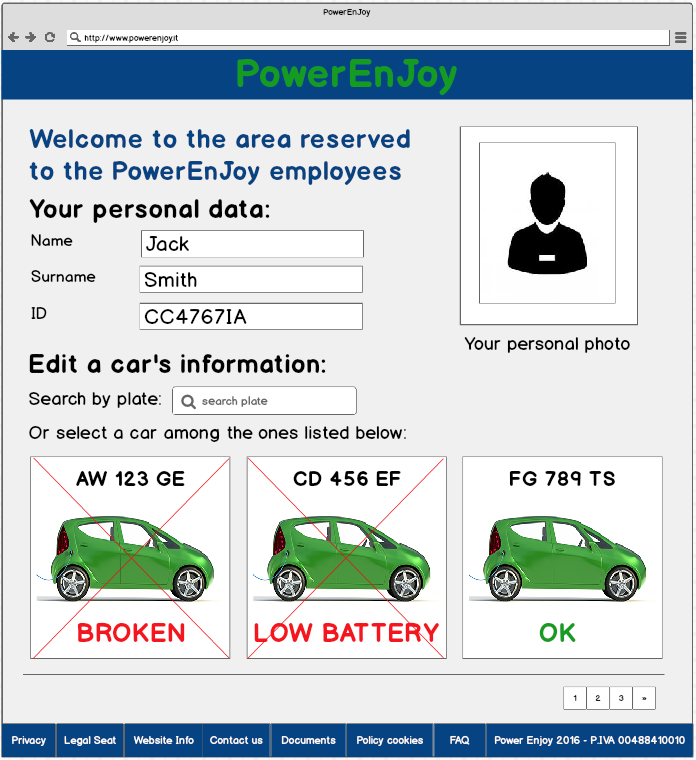
\includegraphics[width=1\textwidth]{EmployeePersonalPage}
	\end{figure}
	\newpage
	\item Employee manages a car's information:
	\begin{figure}[H]
		\centering
		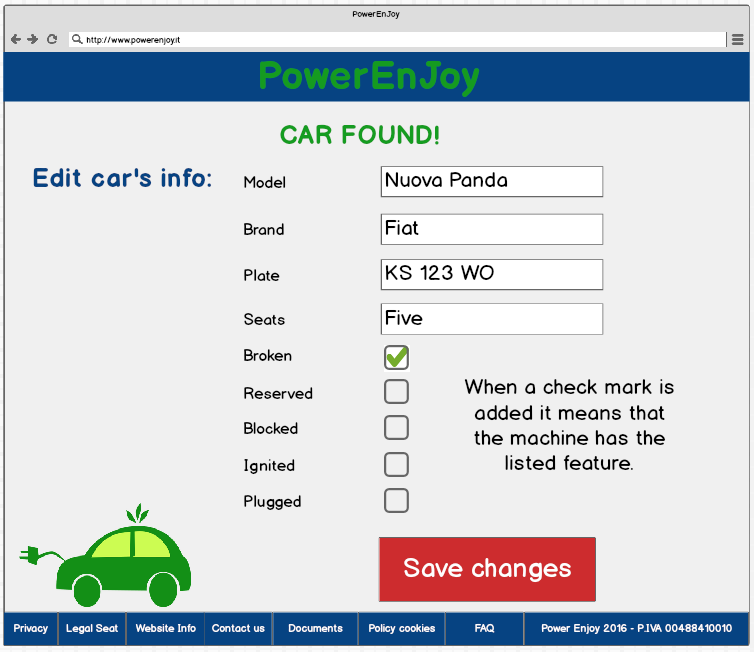
\includegraphics[width=1\textwidth]{EmployeeManagesCarInfo}
	\end{figure}
\end{itemize}
\newpage
\subsubsection{Car}
\begin{itemize}
	\item Car screen asking for destination:
	\begin{figure}[H]
		\centering
		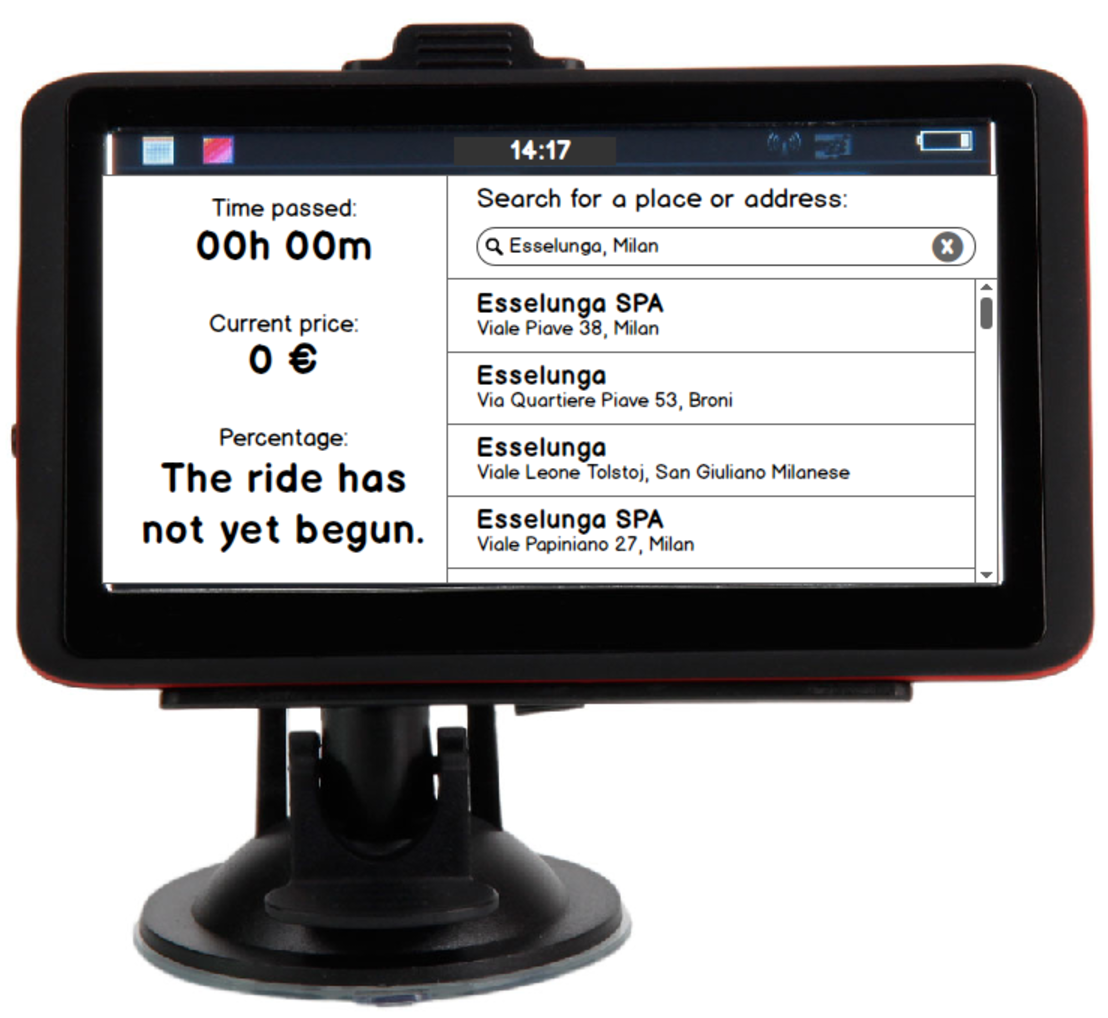
\includegraphics[width=1\textwidth]{Car_screen_where}
	\end{figure}
\newpage
	\item Car screen with map and information about the ride:
	\begin{figure}[H]
		\centering
		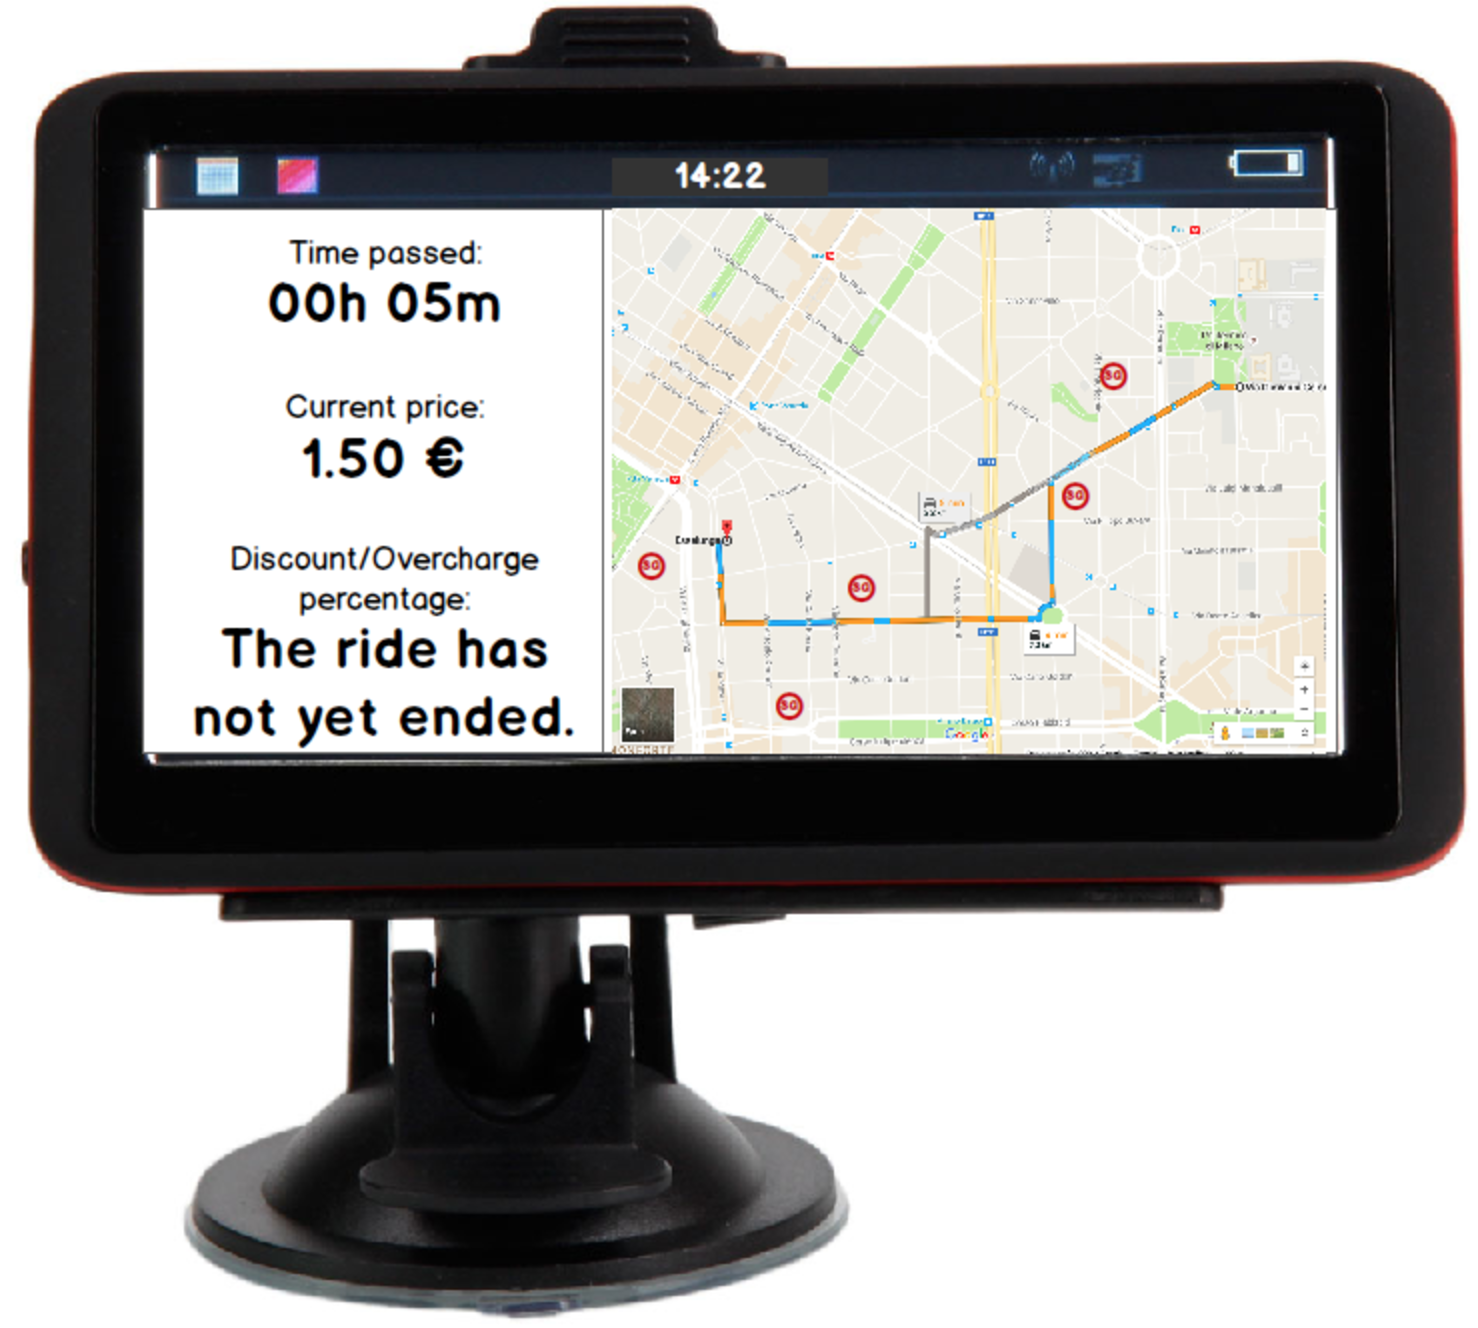
\includegraphics[width=1\textwidth]{Car_screen}
	\end{figure}
\newpage
\item Car screen after the destination is reached:
\begin{figure}[H]
	\centering
	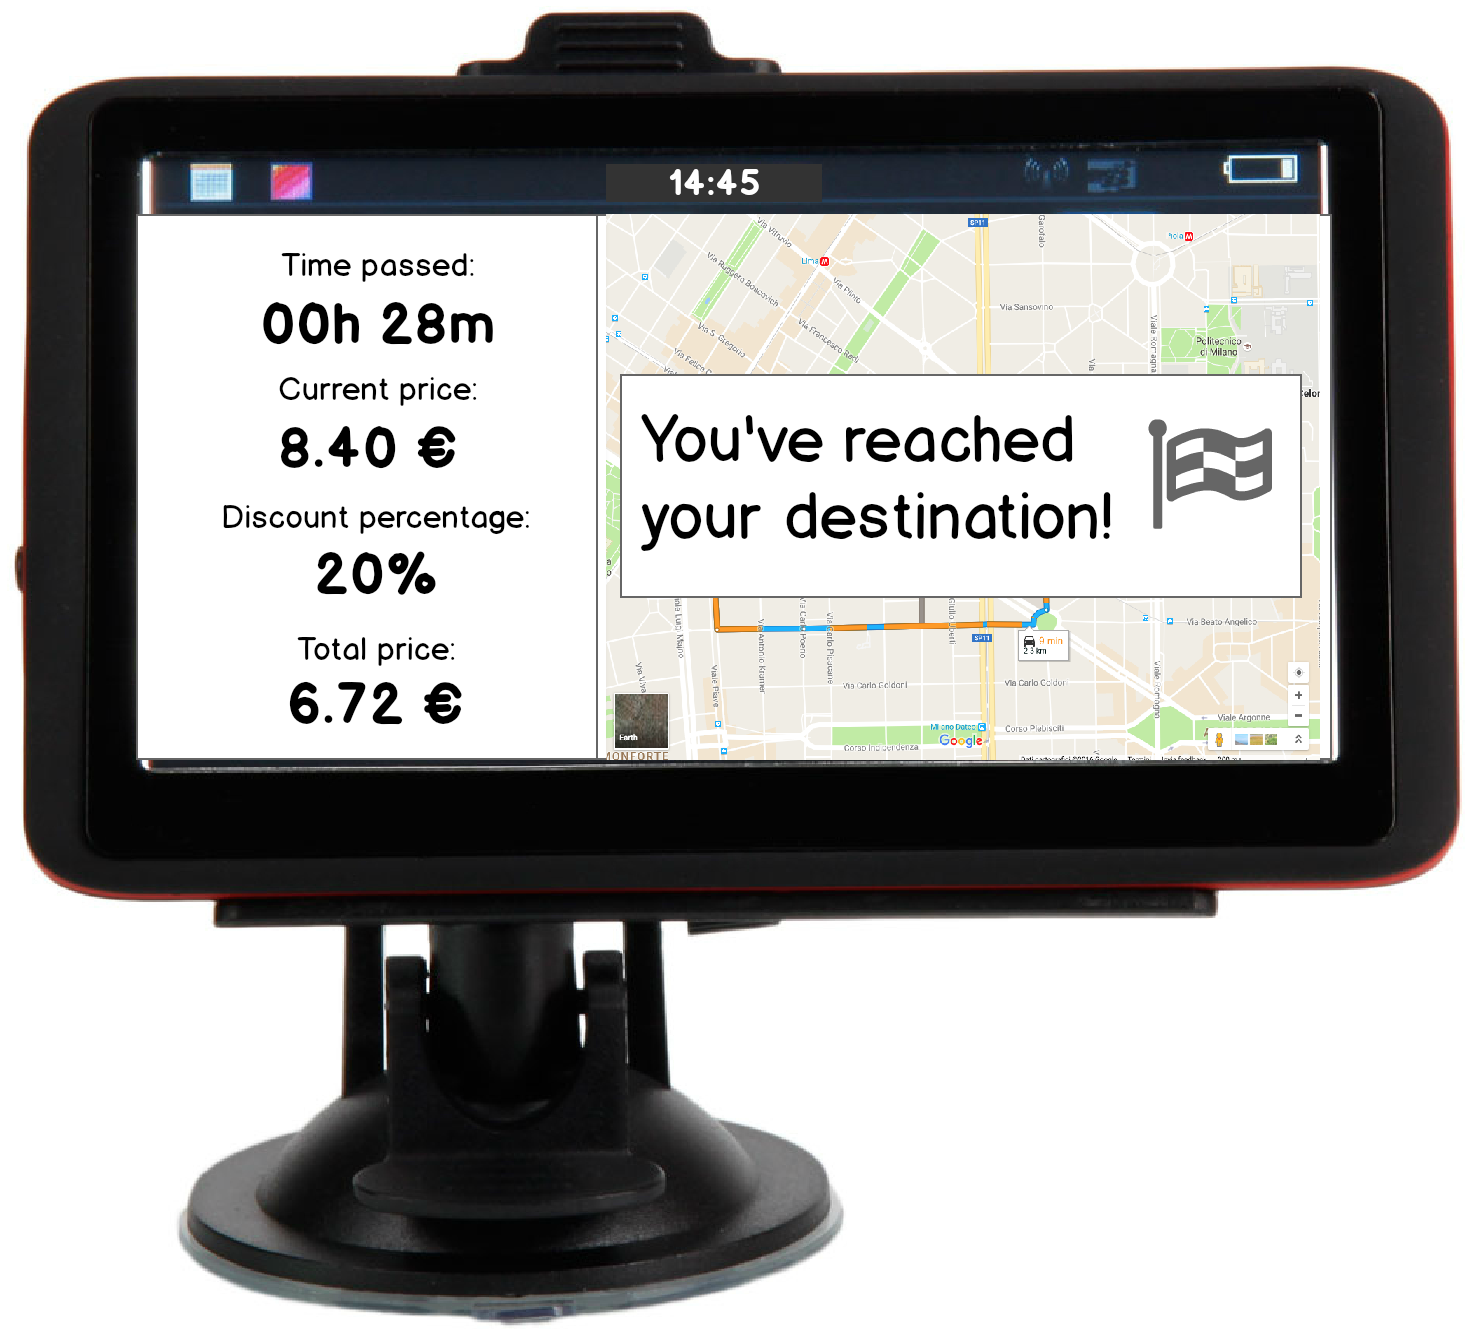
\includegraphics[width=1\textwidth]{Car_screen_destination}
\end{figure}
\end{itemize}
\newpage
\subsubsection{Architectural considerations}
We will use the following technologies:
\begin{itemize}
	\item \textbf{MySQL}, for the storage of all the information related to both the PowerEnJoy application and the users.
	\item \textbf{Mapping service}, to keep track of the position of both cars and registered users (only the ones who allow it). 
	\item \textbf{PHP}, to build the back-end of the application. 
	\item \textbf{JavaScript, HTML, CSS} and \textbf{Bootstrap}, to create a responsive and well-designed website.
	\item \textbf{PhoneGap}, to create a responsive mobile application. 
	\item Modern browser with JavaScript and AJAX support.
	\item \textbf{Java} for Android and iOS apps, using original SDK.
	\item Internet/Ethernet connection for data communication.
	\item \textbf{SMTP (Simple Mail Transfer Protocol)}, to transfer emails from a server to another with a point-to-point connection. 
\end{itemize}